\chapter{Evaluation}
\label{cap:Eval}

Im vorhergegangenen Kapitel wurde die Implementierung der neuronalen Netze beschrieben.
Nun wird in diesem Kapitel betrachtet, wie gut die Ergebnisse sind, die von diesen Netzen geliefert werden.
Dazu wird zunächst beschrieben auf was für einem System das Training und die Evaluation durchgeführt wurde.
Es werden mehrere, bereits aus dem Stand der Technik bekannte Modelle beschrieben, die dann mit den Ergebnissen der neuronalen Netze 
verglichen werden.
Anschließend werden diese Ergebnisse diskutiert.
% \todo[inline]{Im vorhergegangenen Kapitel wurde beschrieben, [wie die Netze designed wurde]
% Jetzt bewerten wie gut sie das eigentlich mache.}

\section{System}

Alle in dieser Arbeit vorgestellten Netze wurden auf einem Ubuntu 18.04 Linux System trainiert und evaluiert.
Dieses verfügt über einen Intel i7-7700k CPU mit \SI{4.20}{\giga\hertz}, eine NVIDIA GeForce 1080Ti Grafikkarte mit \SI{11}{\giga\byte}~GDDR5X
und \SI{32}{\giga\byte}~RAM. 

\todo[inline]{muss da noch irgendwie mehr dazu?}

\section{Vergleichsmodelle}

% \color{blue}
% Notation und Definition bei allen diesen Modellen nach Florian's Diss \cite{Pfaff2018}, mit Ausnahme von Average Acceleration.
% Sei \(x(t)\) die Position des Partikels entlang der Bewegungsrichtung in Abhängigkeit von der Zeit
% (continuous-time equation).
% Sei \( y(t)\) die Position des Partikels orthogonal zur Bewegungsrichtung in Abhängigkeit von der Zeit.
% \(t^{\text{Last}}\) ist der Zeitpunkt der Beobachtung des letzten Features.
% % Sei \(\Delta t =  t - t^{\text{Last}}\).

% Vergleich über Boxplots: Balken: 25\%-Quantil bis 75\%-Quantil.
% Roter Balken ist der Median. Der obere und der untere Whisker 
% gehen bis zum höchsten bzw. niedrigsten Wert, der nicht mehr als 2.7 Standardabweichungen vom Median abweicht
% Die Outlier werden nicht abgebildet.

% \color{black}

In diesem Abschnitt sollen einige der existierenden Modelle detaillierter beschrieben werden mit denen die Ergebnisse der Neuronalen Netze nun verglichen werden.
Diese Modelle wurden schon in Abschnitt~\ref{cap:relWork} erwähnt, dort aber ohne die Berechnung zu erklären.
Mit Ausnahme des \textit{Average Acceleration} Modells stammen sie alle aus \cite{Pfaff2018} und sowohl Definition als auch Notation wurden von dort übernommen.
Dabei seien \(x\) die Achse entlang der Bewegungsrichtung des Förderbands und \(y\) die Achse orthogonal zur Bewegungsrichtung des Förderbands.
Zeitdiskreten Messungen entlang der einzelnen Achsen werden als \(\mathsf{x}_t\) beziehungsweise \(\mathsf{y}_t\) dargestellt.
Die daraus rekonstruierten zeitkontinuierlichen Positionsgleichungen werden als \(\mathsf{x}(t)\) beziehungsweise \(\mathsf{y}(t)\) bezeichnet.
Sei \(t^{\text{Last}}\) der Zeitpunkt der Beobachtung des aktuellsten Features und \(\mathsf{x}^{\text{Last}}\) und \(\mathsf{y}^{\text{Last}}\) die dazugehörigen Positionen entlang der beiden Achsen.
Sei \(\mathsf{x}^{\text{PredTo}}\) die Position des Druckluftdüsenarrays entlang der \(x\)-Achse.
Sei \(t^{\text{Pred}}\) der Zeitpunkt an dem ein Partikel den Druckluftdüsenarray passiert.
Sei \(\mathsf{y}^{\text{Pred}} = \mathsf{y}(t^{\text{Pred}})\) die Position entlang der \(y\)-Achse an dem der Partikel den Druckluftdüsenarray passiert.
\(\Delta t = t^{\text{Pred}} - t^{\text{Last}} \) und \(\mathsf{y}^{\text{Pred}}\) dementsprechen den Labels der einzelnen Feature-Label-Paare für das Separator-Netz.
\(\mathsf{x}(t^{\text{Last}} + 1)\) und \(\mathsf{y}(t^{\text{Last}} + 1)\) entsprechen den Labels der Feature-Label-Paare für das NextStep-Netz.
Die verschiedenen Modelle können nun ebenso wie die Ergebnisse der verschiedenen Netze bewertet werden, 
indem man die Abweichung zwischen dem Ergebnis in dem Modell und der Ground Truth in den Feature-Label-Paaren bestimmt.
\todo[inline]{Das formatting hier ist total schlecht - überlegen wie ich das gut machen kann.}


Für Modelle, die unabhängig von der Beschleunigung der Teilchen sind, ist der Zustandsvektor als 
% 
\begin{equation} \label{eq:definitionCV}
    \vx(t) = 
    \begin{bmatrix}
        \mathsf{x}(t) \\
        \dot{\mathsf{x}}(t) \\
        \mathsf{y}(t) \\
        \dot{\mathsf{y}}(t)
       \end{bmatrix} 
\end{equation}
% 
definiert.
Für Modelle, die die Beschleunigung der Teilchen mit einbeziehen, ist der Zustandsvektor folgendermaßen definiert:
% 
\begin{equation} \label{eq:definitionCA}
    \vx(t) = 
    \begin{bmatrix}
        \mathsf{x}(t) \\
        \dot{\mathsf{x}}(t) \\
        \ddot{\mathsf{x}}(t) \\
        \mathsf{y}(t) \\
        \dot{\mathsf{y}}(t) \\
        \ddot{\mathsf{y}}(t)
       \end{bmatrix} 
\end{equation}
% 
\todo[inline]{Irgendwo irgendwas dazu sagen, wie es mutmaßlich wirklich ist?
Geschwindigkeit Förderband ist eine obere Grenze - bis dahin beschleunigen, dann konstante Geschwindigkeit.
Wie schnell diese Geschwindigkeit erreicht wird hängt von der Art des Schüttguts ab.
Je länger das Band desto mehr Zeit hat das Schüttgut sich an die Geschwindigkeit anzupassen.}

\paragraph{Constant Velocity Modell}

Das Constant Velocity (CV) Modell arbeitet unter der Annahme, dass sich Partikel, 
abgesehen von einem Rauschterm, mit einer konstanten Geschwindigkeit bewegen.
Es kann mittels folgender Differenzialgleichung dargestellt werden.

\begin{equation*} \label{eq:speedCV}
    \dot{\vx}(t) = \mat{A}\vx(t), \quad \mat{A} = 
    \begin{bmatrix}
        0 & 1 & 0 & 0 \\
        0 & 0 & 0 & 0 \\
        0 & 0 & 0 & 1\\
        0 & 0 & 0 & 0
    \end{bmatrix} 
\end{equation*}

Daraus folgen die Positionsgleichungen 
\begin{equation*}
    \mathsf{x}(t) = \mathsf{x}^{\text{Last}} + (t - t^{\text{Last}})\dot{\mathsf{x}}^{\text{Last}} \: ,
\end{equation*}
\begin{equation*}
    \mathsf{y}(t) = \mathsf{y}^{\text{Last}} + (t - t^{\text{Last}})\dot{\mathsf{y}}^{\text{Last}}
\end{equation*}
% 
entlang der einzelnen Achsen.
Für das NextStep-Szenario ergibt sich die Prädiktionen mittels des CV Modells also aus
\begin{equation*}
    \mathsf{x}(t\hitext{Last}+1) = \mathsf{x}^{\text{Last}} + \dot{\mathsf{x}}^{\text{Last}} \: ,
\end{equation*}
\begin{equation}\label{eq:cvyp}
    \mathsf{y}(t\hitext{Last}+1) = \mathsf{y}^{\text{Last}} + \dot{\mathsf{y}}^{\text{Last}} \: .
\end{equation}

Für das Separator-Szenario lösen wir die Gleichung 
% 
\begin{equation*}
    \mathsf{x}^{\text{PredTo}} = \mathsf{x}^{\text{Last}} + (t - t^{\text{Last}})\dot{\mathsf{x}}^{\text{Last}}
\end{equation*}
% 
für \(t\) um  \(t^{\text{Pred}}\) zu erhalten.
Durch das Einsetzen von \(t^{\text{Pred}}\) in \eqref{eq:cvyp} ergibt sich \(\mathsf{y}^{\text{Pred}}\).

\paragraph{Constant Acceleration Modell}

Im Constant Acceleration (CA) Modell wird davon ausgegangen, dass das das Teilchen mit einer konstanten Beschleunigung schneller wird.
Es kann mittels folgender Differenzialgleichung dargestellt werden.

\begin{align*} \label{eq:speedCV}
    \dot{\vx}(t) = \mat{A}\vx(t), \quad \mat{A} = 
    \begin{bmatrix}
        \mat{A}_x & \boldsymbol{0} \\
        \boldsymbol{0} & \mat{A}_y
    \end{bmatrix} 
    , \quad
    \mat{A}_x = \mat{A}_y = 
    \begin{bmatrix}
        0 & 1 & 0 \\
        0 & 0 & 1 \\
        0 & 0 & 0
    \end{bmatrix} 
\end{align*}

Analog zum Constant Velocity Modell können daraus die Positionsgleichungen 
% 
\begin{equation*}
    \mathsf{x}(t) = \mathsf{x}^{\text{Last}} + (t - t^{\text{Last}})\dot{\mathsf{x}}^{\text{Last}} 
    + \frac{1}{2} (t - t^{\text{Last}})^2 \: \ddot{\mathsf{x}}^{\text{Last}} \: , 
\end{equation*}
\begin{equation*}
    \mathsf{y}(t) = \mathsf{y}^{\text{Last}} + (t - t^{\text{Last}})\dot{\mathsf{y}}^{\text{Last}}
    + \frac{1}{2} (t - t^{\text{Last}})^2 \: \ddot{\mathsf{y}}^{\text{Last}}
\end{equation*}
% 
abgeleitet werden.
Genau wie beim Constant Velocity Modell werden nun jeweils entweder die Gleichung für \(t = \text{Last} + 1\) gelöst 
um die Prädiktion für den NextStep-Fall oder \(\Delta t \) und daraus \(\mathsf{y}^{\text{Pred}}\) für den Separator-Fall gelöst.


\paragraph{Bias-Corrected Constant Velocity Modell}

In \cite{Pfaff2018} wurden weitere szenariospezifische Bewegungsmodelle beschrieben, die insbesondere die Qualität der zeitlichen Prädiktion für den Separator-Fall verbessern.
Das erste von diesen Modellen, das hier zum Vergleich mit den Ergebnissen der neuronalen Netze betrachtet werden soll, ist eine Verbesserung des Constant Velocity Modells und wird als Bias-Corrected Constant Velocity (CVBC) Modell bezeichnet.
Durch das Bestimmen des durchschnittlichen Bias bezüglich der Ankunftszeit der Partikel am Druckluftdüsenarray in den Trainingsdaten und das Abziehen des selben vom der Prädiktion der Testdaten kann die Qualität dieser Prädiktion verbessert werden.
Dieser neue Wert kann nun für die Ortsprädiktion benutzt werden und verbessert auch diese.
Damit ergibt sich für die vorhergesagte Ankunftszeit
% 
\begin{equation*}
    t\hitext{Pred, CVBC} = t\hitext{Pred, CV} - t\hitext{Bias} \, ,
\end{equation*}
% 
wobei \(t\hitext{Bias}\) den durchschnittlichen Bias bezüglich der Ankunftszeit bezeichnet.
Analog zum unveränderterten Constant Velocity Modell erhält man nun durch das Einsetzen von \(t^{\text{Pred, CVBC}}\) in \eqref{eq:cvyp} erneut \(\mathsf{y}^{\text{Pred, CVBC}}\).
Die Verbesserung der prädizierten Zeit führt ebenfalls zu einer Verbesserung des prädizierten Orts.


\paragraph{Average Acceleration Modell}

% \color{blue}
% Für alle Elemente des Trainingssets: Bestimme die Beschleunigungen.
% Sei \(\ddot{x}\hitext{Median}\) der Median von all diesen Beschleunigungen.
% Benutze ihn als Beschleunigung wie im CA Modell

% (Basicly CV Modell + eine Beschleunigung basierend auf den Trainingsdaten)

% \todo[inline]{überhaupt erwähnen? Er ist way better als er irgendein right hat}
% \color{black}

Das Average Acceleration (AA) Modell ist eine Erweiterung des CVBC-Modells.
Anstatt die durchschnittliche Abweichung der prädizierten Zeit in den Trainingsdaten auf die prädizierte Zeit zu addieren, wird angenommen, 
dass diese Abweichung aus einer nicht betrachteten Beschleunigung resultiert.
Diese Beschleunigung wird mutmaßlich vom Band verursacht werden und alle Partikel mehr oder weniger ähnlich betreffen.
Deshalb wird die Beschleunigung des Partikels in allen Feature-Label-Paaren des Trainingssets bestimmt
und von diesen der Median \(\ddot{ \mathsf{x}}^{\text{Median}}\) gewählt als eine einheitliche Beschleunigung, die zum CV Modell hinzugefügt wird.
Es folgt die Positionsgleichung
\begin{equation*}
    \mathsf{x}(t) =  \mathsf{x}^{\text{Last}} + (t - t^{\text{Last}}) \: \dot{ \mathsf{x}}^{\text{Last}} 
    + \frac{1}{2} (t - t^{\text{Last}})^2 \: \ddot{ \mathsf{x}}^{\text{Median}} \: ,
\end{equation*}
% 
die wir für \(\mathsf{x}(t) =  \mathsf{x}^{\text{PredTo}}\) nach \(t\) lösen.


\paragraph{Identical Acceleration Modell}

% \color{blue}
% Upgrade zu CVBC: Correction Term, der den die Letzte Position des Partikels einbezieht.\\
% Annahme: Abweichungen bezüglich dem Zeit Label wird von einer zusätzlichen Beschleunigung verursacht.
% \color{black}

Das Identical Acceleration (IA) Modell ist ebenfalls eine Verbesserung des CVBC-Modells. 
Bei diesem werden die Korrekturterme, die als Beschleunigung auf die Positionsgleichungen addiert werden, nicht unabhängig von der letzten Position des Partikels bestimmt, sondern beziehen diese mit ein.
Wie oben wird hierbei die Annahme getroffen, dass die zusätzliche Beschleunigung, die für die zeitliche Abweichung sorgt, für alle Partikel ungefähr gleich ist.
Die Bestimmung dieser Korrekturterme ist jedoch unterschiedlich.
Für die Feature-Label-Paare des Trainingssets hat man man Zugang zu der Ground Truth, wann die Partikel das Druckluftdüsenarray passieren.

Dementsprechen lösen wir für jedes Partikel \( i\) aus dem Trainingsset die Gleichung
% 
\begin{equation*}
    \mathsf{x}\hitext{PredTo} =  \mathsf{x}\hitext{Last, \(i\)} + (t\hitext{GT, \(i\)} - t\hitext{Last, \(i\)}) 
    \: \dot{ \mathsf{x}}\hitext{Last, \(i\)}
    + \frac{1}{2}(t\hitext{GT, \(i\)} - t\hitext{Last, \(i\)})^2 \: \ddot{ \mathsf{x}}\hitext{Optimal, \(i\)}
\end{equation*}
% 
um herauszufinden, mit welcher zusätzlichen Beschleunigung \(\ddot{ \mathsf{x}}\hitext{Optimal, \(i\)}\) es optimal die Zeit,
die es noch braucht, vorhersagen würde.
Nun sei \(\ddot{ \mathsf{x}}\hitext{Avg}\) der Durchschnitt von allen \(\ddot{ \mathsf{x}}\hitext{Optimal, \(i\)}\).
Für die Partikel des Testsets werden die Zeit und der Ort des Passierens des Druckluftdüsenarrays nun basierend auf deren 
beobachteter Geschwindigkeit \(\dot{ \mathsf{x}}^{\text{Last}}\) und der errechneten Beschleunigung \(\ddot{ \mathsf{x}}\hitext{Avg}\) berechnet.
Die Zeitprädiktion \(t\hitext{Pred}\) wird bestimmt indem wir
% 
\begin{equation*}
    \mathsf{x}(t) =  \mathsf{x}^{\text{Last}} + (t - t^{\text{Last}}) \: \dot{ \mathsf{x}}^{\text{Last}} 
    + \frac{1}{2} (t - t^{\text{Last}})^2 \: \ddot{ \mathsf{x}}\hitext{Avg}
\end{equation*}
% 
nach \(t\) lösen.

\paragraph{Visualisierung}

Der Vergleich zwischen unterschiedlichen Modelle wird mittels sogenannter Boxplots visualisiert.
Die fünf relevanten Charakteristiken, die in einem Boxplot dargestellt werden sind 
der Median, das untere und obere Quartil sowie zwei sogenannte "Antennen" oder auch "Whisker", die die Position den letzten Datenpunkt innerhalb des 1.5-fachen Interquartilsabstands beschreiben.
Die Position des Medians wird durch eine rote Linie verdeutlicht.
Die namensgebende Box ist zwischen dem unteren und dem oberen Quartil aufgespannt.
Für die Darstellung in dieser Arbeit wurde darauf verzichtet Ausreißer außerhalb der Antennen abzubilden.



% \todo{fertig machen}

\section{Next Step}

% \color{blue}
% Netz Variante 1: den nächsten Schritt vorhersagen
% \(\Delta t \) ist immer 1.


% Für Nextstep gesucht: \( \mathsf{x}(t^{\text{Last}} + 1)\)

% \todo[inline]{Latex Tabelle des pandas Dataframe mit den Spalten GroundtruthX, GroundtruthY, 
% NNPrädiktionX, NNPrädiktion, CV\_X, CV\_Y, CA\_X, CA\_Y}
% \color{black}

In dieser Sektion soll das Ergebnis der NextStep-Netze in verschiedenen Szenarien betrachtet werden.
Als Evaluationskriterium für die NextStep-Netze wurde die Euklidische Distanz zwischen der Prädiktion des Modell und der Ground Truth gewählt.
Der Gesamtfehler \(\varepsilon\hitext{Total} \) ist also durch 

\begin{align*}
    \mathsf{x}\hitext{Err} &=  \mathsf{x}\hitext{Pred} -  \mathsf{x}\hitext{GT} \: ,\\
    \mathsf{y}\hitext{Err} &=  \mathsf{y}\hitext{Pred} -  \mathsf{y}\hitext{GT} \: ,\\
    \varepsilon\hitext{Total} &= \sqrt{ \mathsf{x}\hitext{Err}^2 +  \mathsf{y}\hitext{Err}^2}
\end{align*}

definiert. Verglichen wird das NextStep-Netz mit einem Constant Velocity Modell und einen Constant Acceleration Modell.

% Die im Rahmen dieser Arbeit trainierten neuronalen Netze haben in allen untersuchten Szenarien bessere Ergebnisse als die beiden Vergleichsmodelle geliefert.
% \todo{kann man das bei den Simulierten Zylindern so sagen?}
Repräsentativ für ihre jeweiligen Szenariokategorien sind in Abbildung~\ref{subfig:RealSpheresBoxplot} die Boxplots für die selbst aufgenommenen Kugeln auf dem Förderband,
und in Abbildung~\ref{subfig:SimSpheresBoxplot} die Boxplots für die mittels DEM simulierten Kugeln zu sehen.
In beiden Fällen ist das Ergebnis des Neuronalen Netzes besser als die Vergleichsmodelle
Es ist auffällig, dass bei den simulierten Daten das CA Modell besser als das CV Modell ist, während es im anderen Fall umgekehrt ist.
Das ist auf die die höhere Bandgeschwindigkeit bei der Simulation zurückzuführen. 
In Abbildung~\ref{fig:RealSpheresHistogram} sieht man das Fehlerhistogramm, dass zu Abbildung~\ref{subfig:RealSpheresBoxplot} gehört.
Es ist zu erkennen, dass die Prädiktionen des neuronalen Netz sowohl einen besseren Erwartungswert als auch eine geringere Standardabweichungen als die Vergleichsmodelle hat.


Die Boxplots und Histogramme der übrigen Szenarien sind im Anhang zu finden.
\todo[inline]{hier könnte ich noch mehr schreiben zu verschiedenen anderen Szenarien, wenn es notwendig sein sollte.}
\todo[inline]{NextStep Boxplot schön machen ohne titel und in mm}

\begin{figure}[htbp]
    \centering
	
	\begin{subfigure}[t]{0.8\textwidth}
		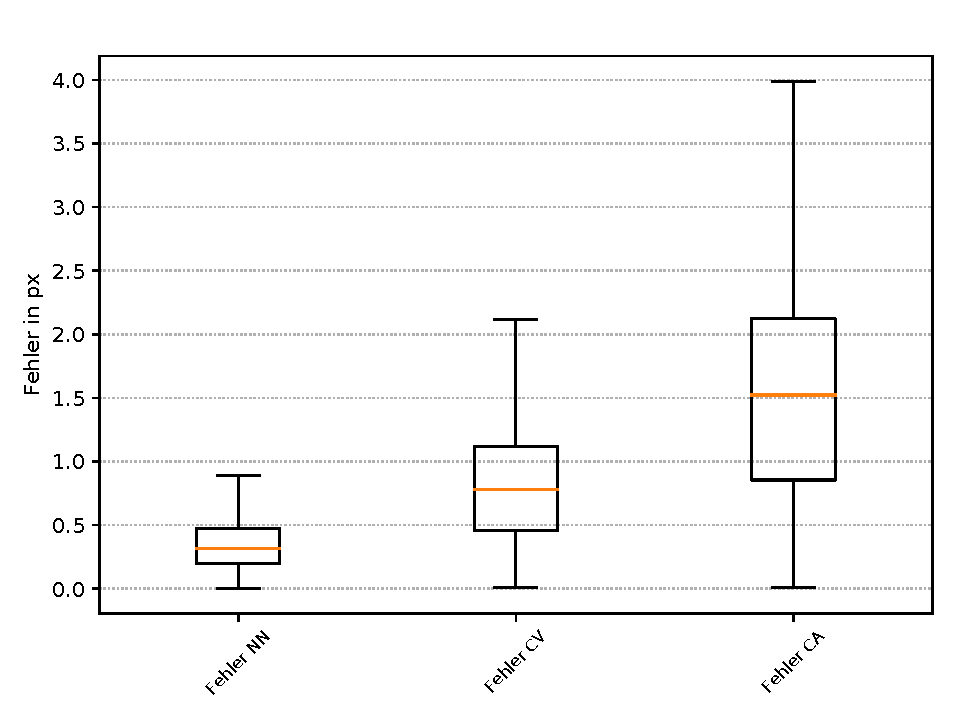
\includegraphics[width=\textwidth]{RealSpheres-evaluation_NextStep_LocationError_2018-12-10_18-42-20.pdf}
		\caption{Boxplots für die NextStep-Ergebnisse der selbst aufgenommenen Kugeln auf dem Förderband.}
		\label{subfig:RealSpheresBoxplot}
	\end{subfigure}
    % \quad
    \vskip\baselineskip
	\begin{subfigure}[t]{0.8\textwidth}
		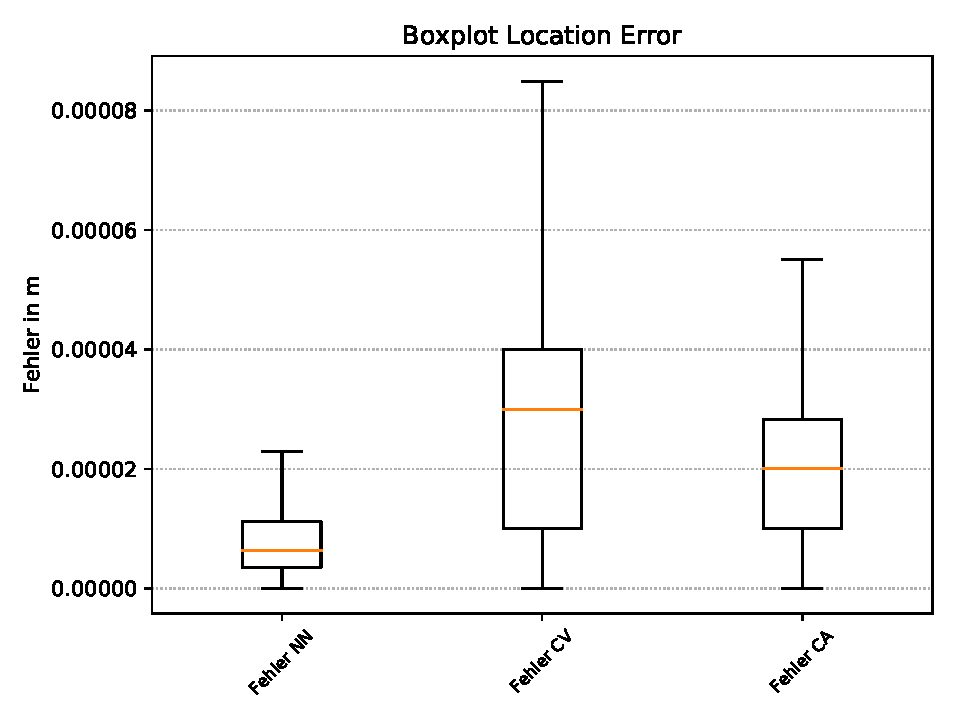
\includegraphics[width=\textwidth]{SimulatedSpheres-evaluation_NextStep_LocationError_2018-12-10_19-09-25.pdf}
		\caption{Boxplots für die NextStep-Ergebnisse der Kugeln aus dem DEM-Datensatz.}
		\label{subfig:SimSpheresBoxplot}
	\end{subfigure}
	
	\caption{Visualisierung der Ergebnisse für die realen und simulierten Kugeln mit NextStep-Netzen}
	\label{fig:BoxplotsNextStep}
\end{figure}

\begin{figure}[h]
    \centering
    % \missingfigure{Boxplots Result NeuralNets NextStep}
	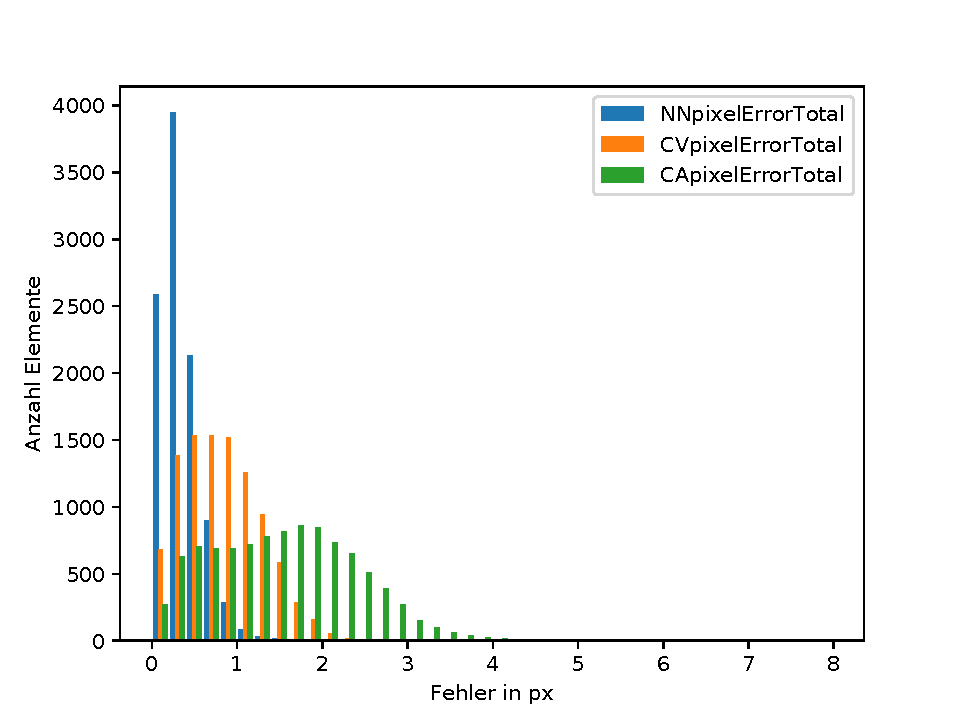
\includegraphics[width=0.8\textwidth]{RealSpheres-evaluation_NextStep_ErrorHistogram_2018-12-10_18-42-20.pdf}
	\caption{Histogramm der Fehler für die NextStep-Ergebnisse der selbst aufgenommenen Kugeln auf dem Förderband.}
	\label{fig:RealSpheresHistogram}
\end{figure}




% Bemerkenswert schlecht war das Ergebnis allerdings bei dem DEM Zylinder Datensatz.
% Es konnte nicht abschließend geklärt werden warum dies der Fall ist, vorallem da die Ergebnisse auf den realen Zylindern, wie in Abbildung TODO zu sehen, deutlich besser waren. 
% Man könnte jedoch vermuten, dass es eine Kombination der folgende Umstände ist.
% Bei den Zylindern hängt ihre Bewegung und die Aufnahme von Bewegungsenergie vom Förderband mehr von ihrer Orientierung ab, als bei den anderen Schüttgütern.
% Diese ist nicht aus den Eingabefeatures ersichtlich - potenziell wäre es bei diesem Szenario also lohnenswert mehr als nur die Mittelpunkte als Feature zu betrachten.
% Die höhere Bandgeschwindigkeit in der Simulation als in den Realdaten könnte diesen Effekt verstärkt haben.
% Auch könnte die höhere Schüttgutdichte auf dem Förderband darauf einen Einfluss gehabt haben.



% \color{blue}
% - CV, CA
% - Ergebnis Netz

% Vergleich Realdaten und simulierte Daten.
% Realdaten mit ungefähr \SI{1.1}{\meter\per\second} während Simulierte mit \SI{1.5}{\metre\per\second} Bandgeschwindigkeit 

% \color{black}

\section{Separator}

% \color{blue}
% CV, CA quasi wie oben.
% zusätzlich: CVBC, AA und IA

% - Ergebnis NN
% \color{black}



In dieser Sektion sollen nun die Ergebnisse der Separator-Netze in verschiedenen Szenarien betrachtet werden.
% Im Gegensatz zu diesen können die beiden Labelelemente nicht in einem gemeinsamen Evaluationskriterium zusammengefasst werden.
Hier wird  die zeitliche Abweichung vom prädizierten Kontaktzeitpunkt mit dem Druckluftdüsenarray und die örtliche Abweichung des Schnittpunkts des Bahn des Partikels mit dem Druckluftdüsenarray separat betrachtet.
Wie bei den NextStep-Netzen werden ein Constant Velocity- und ein Constant Acceleration Modell 
als Vergleichsmodelle benutzt. 
Zusätzlich werden noch mehr Vergleichsmodelle hinzugezogen. 
Das Bias-Corrected Constant Velocity Modell liefert eine sowohl Prädiktion für den Zeit als auch für den Ort.
Die Average Acceleration und Identical Acceleration Modelle werden nur für die zeitliche Prädiktion zum Vergleich herangezogen.

Die Evaluation, die hier durchgeführt wurde erfolgt auf folgendem Szenario.
Als Trainingsdaten wurden nur das jeweils letzte Feature-Label-Paar eines Tracks benutzt, bevor das entsprechende Partikel die Prädiktionsphase verlässt.
Es wäre in der Zukunft möglich auf allen möglichen Feature-Label-Paaren zu trainieren um zu erreichen, dass der Ausgangspunkt verschoben werden kann ohne das Netz neu trainieren zu müssen.
\todo{Hier weg und dafür in den Ausblick?}  
Für die DEM-Datensätze wurde von \(x = \SI{0.55}{\meter}\) nach \(x = \SI{0.70}{\meter}\) prädiziert, also \SI{15}{\centi\meter} nach vorne.
Da der gesamte Bildausschnitt der selbst aufgenommenen Daten weniger als \SI{15}{\centi\meter} entlang der Bewegungsrichtung misst, musste diese Distanz reduziert werden.
Die auf den selbst gesammelten Daten trainierten Netze prädizieren von \(y = \SI{800}{\px}\) nach \(y = \SI{1550}{\px}\), also eine Distanz von \SI{750}{\px}.
\todo{hier umrechnung in cm dazumachen? ungefähr 4.5 cm}


Die Ergebnisse auf den Separator-Fall werden zweigeteilt als
\begin{align*}
    t\hitext{Err} &=  t\hitext{Pred} -  t\hitext{GT} \: ,\\
    \mathsf{y}\hitext{Err} &=  \mathsf{y}\hitext{Pred} -  \mathsf{y}\hitext{GT}
\end{align*}
definiert.
Im Gegensatz zu dem NextStep-Fall ist es nicht sinnvoll diese Fehler zu einem Gesamtfehler zu kombinieren.
Zusätzlich ist das Vorzeichen der Fehler für die einzelnen Partikel hier relevant.
Für die zeitlichen Fehler bedeutet ein positiver Wert, 
dass das Teilchen früher den Druckluftdüsenarray passiert hat als von dem Modell vorhergesagt. 


Die Ergebnisse der neuronalen Netze für die Separator-Prädiktion sind insgesamt zufriedenstellend.
Sie sind auf allen Datensätzen besser als das CV-Modell, das CV-Modell und das CVBC-Modell.
\todo{Reihenfolge? erst Daten dann schlussfolgerungen}
Auf den beiden simulierten Datensätzen sind die Ergebnisse ein wenig schlechter als das IA-Modell, 
aber deutlich besser als die grundlegenden Modelle und das Bias-Corrected Constant Velocity Modell.
Dies ist in Abbildung~\ref{fig:BoxplotsSimCub} exemplarisch durch die Boxplots der simulierten Plättchen dargestellt.
Zunächst soll der zeitliche Fehler betrachtet werden.
Obwohl der Median des Prädiktionsfehlers einen kleinen Bias ins Positive hat und das untere Quartil tatsächlich positiv ist, werden die Fehler der neuronalen Netzes komplett von denen des CVBC-Modells überdeckt.
Das CV- und das CA-Modell sind beide nocheinmal bedeutend schlechter als das CVBC-Modell.
Das CV-Modell hat einen Bias von beinah zwei ganzen Zeitschritten während das CA-Modell zwar beinah biasfrei ist, ungefähr in der gleichen Größenordnung wie das neuronale Netz, hat es mit Abstand die größte Standardabweichung
Diese ist ungefähr drei mal so groß wie die des Ergebnisses des neuronalen Netzes.
Das beste Modell in diesem Szenario ist das IA-Modell.
Es ist beinah komplett biasfrei und hat die geringste Standardabweichung von allen Modellen.
Bei der Betrachtung des örtlichen Fehlers ist das CA-Modell tatsächlich besser als das CV- oder das CVBC-Modell, aber dennoch deutlich schlechter als das neuronale Netz.
Alle vier Modelle sind beinahe biasfrei, aber der Interquartilsabstands der Ausgabe des neuronalen Netzes sind deutlich geringer. 

\begin{figure}[htbp+]
    \centering
	
	\begin{subfigure}[t]{0.8\textwidth}
		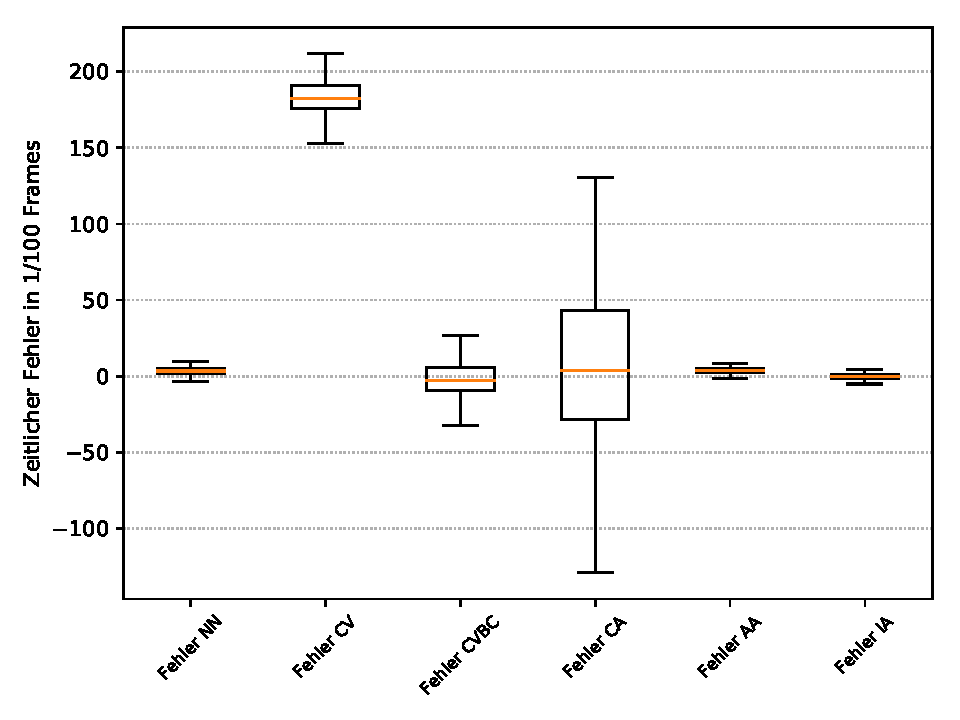
\includegraphics[width=\textwidth]{SimCub-evaluation_Separator_TimeErrorBoxplot_2018-12-11_14-33-22.pdf}
		\caption{Boxplots des zeitlichen Fehlers für die Separator-Ergebnisse der Plättchen aus dem DEM-Datensatz.}
		\label{subfig:SimCubTimeBoxplot}
	\end{subfigure}
    % \quad
    \vskip\baselineskip
	\begin{subfigure}[t]{0.8\textwidth}
		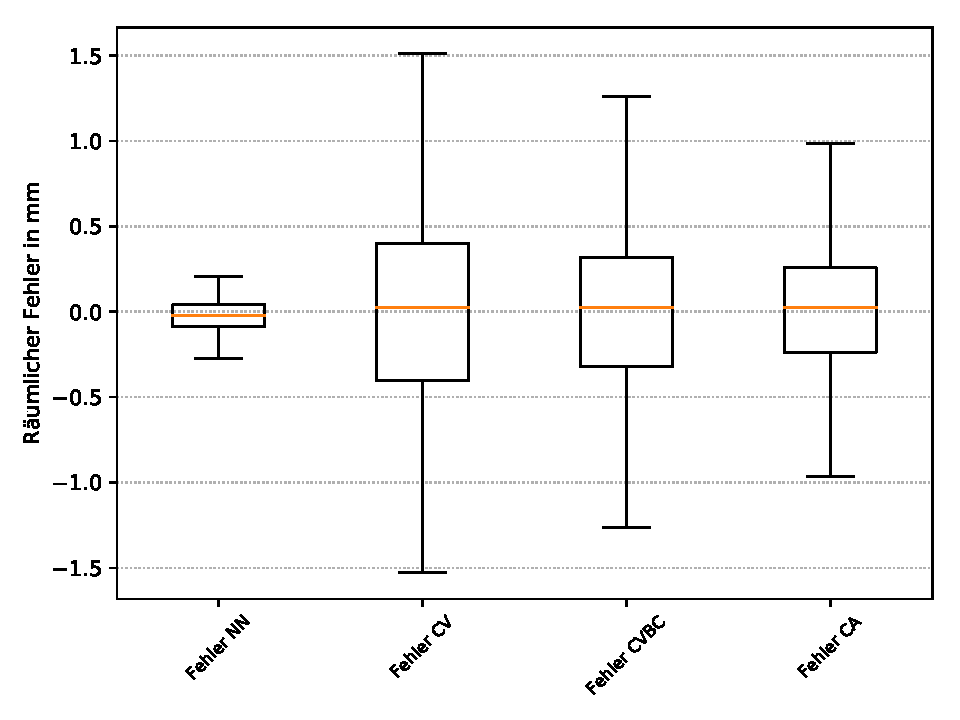
\includegraphics[width=\textwidth]{SimCub-evaluation_Separator_LocationErrorBoxplot_2018-12-11_14-33-22.pdf}
		\caption{Boxplots des örtlichen Fehlers für die Separator-Ergebnisse der Plättchen aus dem DEM-Datensatz.}
		\label{subfig:SimCubLocBoxplot}
	\end{subfigure}
	
	\caption{Visualisierung der Ergebnisse für die Plättchen aus der DEM-Simulation.}
	\label{fig:BoxplotsSimCub}
\end{figure}

Im Vergleich dazu sind die Unterschiede zwischen den verschiedenen Modellen auf den selbst aufgenommenen Daten deutlich kleiner.
Das Constant Velocity Modell schneidet oft beinah so gut 
und bei den Weizenkörnern sogar besser ab, als das Identical Acceleration Modell.
Auf den selbst gesammelten Daten schneidet von den bestehenden Modellen das Bias-Corrected Constant Velocity Modell am besten ab. 
Die neuronalen Netze sind jedoch nocheinmal besser. 
Wenn man die Boxplots der zeitlichen Fehler der verschiedenen Modelle auf dem Weizenkörner-Datensatz der selbst aufgenommenen Daten, dargestellt in Abbildung~\ref{subfig:RealWeizenTimeBoxplot},
im Detail betrachtet gibt es einige Auffälligkeiten. 
Im Gegensatz zu dem in Abbildung~\ref{subfig:SimCubTimeBoxplot} dargestellten Szenario
zeigt der zeitliche Fehler des CV-Modells nur einen geringen Bias, der sogar eher negativ ist.
Während es im bei den simulierten Plättchen so ist, 
dass der Interquartilsabstands des CV-Modells um Faktoren größer ist als der der IA-Modells, ist er hier fast gleich groß.
Tatsächlich unterscheiden sich die Ergebnisse der CV-, CVBC-, AA- und IA- fast nur in ihrem Bias.
Dem gegenüber stehen die Ergebnisse des neuronalen Netz, die fast komplett biasfrei sind und einen merklich kleineren Interquartilsabstands hat als jedes der bestehenden Modelle.
Ähnlich ist es beim räumlichen Fehler, der in Abbildung~\ref{subfig:RealWeizenLocBoxplot} dargestellt ist.
Obwohl die Ergebnisse des neuronalen Netzes einen kleinen Bias haben, wird der Bereich zwischen ihrem oberen und unteren Quartil immer noch komplett überdeckt von der Box des CVBC-Modells, das das beste der Vergleichsmodelle ist.

% \todo[inline]{Resultat verifizieren}
Die Resultate der bestehenden Modelle hängen höchstwahrscheinlich mit der niedrigeren Bandgeschwindigkeit und dem kürzeren Prädiktionsabstand zusammen.
Auch die könnten die unterschiedlichen Verfahren unterschiedlich anfällig gegen das Messrauschen sein, das auf den simulierten Daten nicht existiert.
Für die bestehenden Modelle gilt, dass eine relative Verbesserung der zeitliche Prädiktion zu einer Verbesserung der örtlichen Prädiktion führt,
da die zeitliche Prädiktion benutzt wird um die örtliche zu bestimmen.
Das ist besonders gut in Abbildung~\ref{fig:BoxplotsSimCub} zu erkennen. 
Die Verbesserung der zeitlichen Prädiktion, zu sehen in Abbildung~\ref{subfig:SimCubTimeBoxplot}, zwischen dem CV- und dem CVBC-Modell sorgt auch direkt für eine Verbesserung der örtlichen Prädiktion, zu sehen in Abbildung~\ref{subfig:SimCubLocBoxplot}.
Für die Ausgabe der neuronalen Netze gilt das jedoch nicht. Hier werden beide Ausgaben parallel bestimmt. 

Wie schon für die NextStep-Netze sind die Boxplots und Histogramme der restlichen Szenarien im Anhang zu finden.

\begin{figure}[htbp]
    \centering
	
	\begin{subfigure}[t]{0.8\textwidth}
		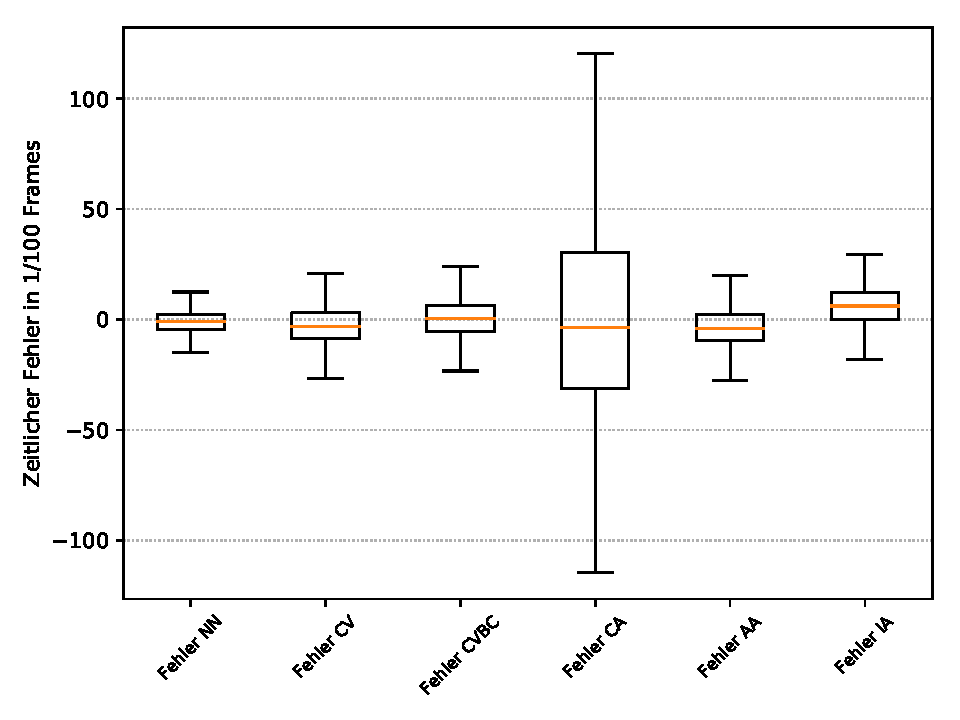
\includegraphics[width=\textwidth]{RealWeizen-evaluation_Separator_TimeErrorBoxplot_2018-12-11_14-09-12.pdf}
		\caption{Boxplots des zeitlichen Fehlers für die Separator-Ergebnisse des Weizenkörnern-Datensatz von den selbst gesammelten Daten.}
		\label{subfig:RealWeizenTimeBoxplot}
	\end{subfigure}
    % \quad
    \vskip\baselineskip
	\begin{subfigure}[t]{0.8\textwidth}
		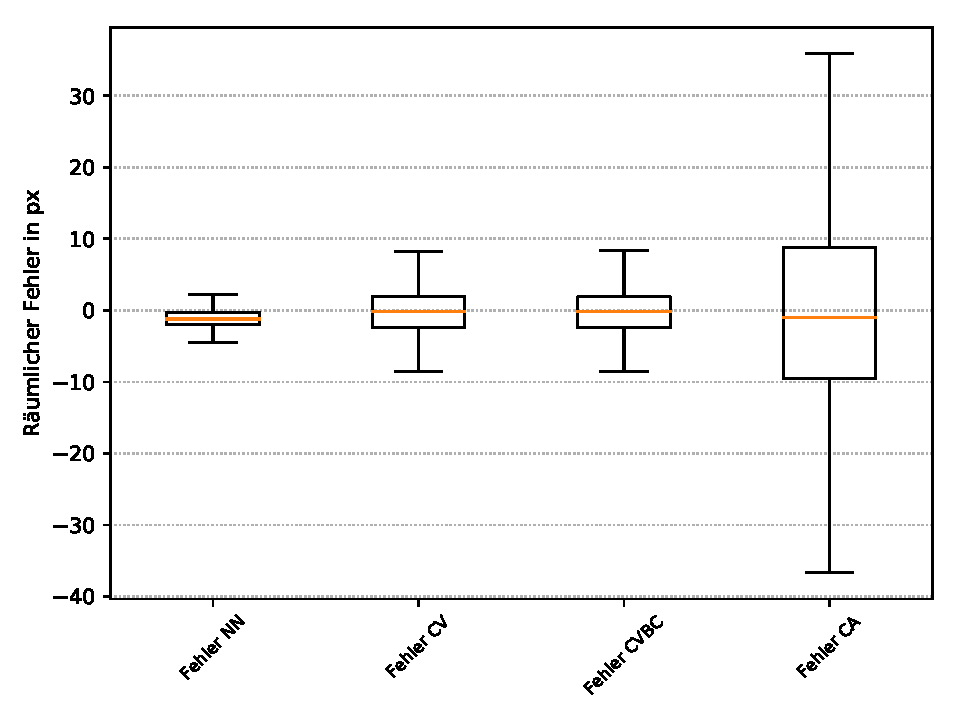
\includegraphics[width=\textwidth]{RealWeizen-evaluation_Separator_LocationErrorBoxplot_2018-12-11_14-09-12.pdf}
		\caption{Boxplots des örtlichen Fehlers für die Separator-Ergebnisse des Weizenkörnern-Datensatz von den selbst gesammelten Daten.}
		\label{subfig:RealWeizenLocBoxplot}
	\end{subfigure}
	
	\caption{Visualisierung der Ergebnisse für den Weizenkörnern-Datensatz von den selbst gesammelten Daten.}
	\label{fig:BoxplotsRealWeizen}
\end{figure}


\section{Zusammenfassung und Diskussion}

\todo[inline]{Einleitung und Zusammenfassung}

Die Tatsache, dass die Separator-Netze auf den DEM-Datensätzen, im Gegensatz zu allen anderen Szenarios,
hinter dem aktuellen Stand der Technik zurück bleiben könnte darauf zurückzuführen sein, 
dass dort verhältnismäßig weniger Trainingsdaten zur Verfügung standen.
Wie bereits in Kapitel~\ref{cap:data} erwähnt, haben DEM-Datensätzen im Vergleich zu den selbst aufgenommenen Daten weniger, aber dafür deutlich längere Tracks.
Für die NextStep-Netze sorgt die größere Länge dazu, dass sogar mehr Feature-Label-Paare aus den DEM-Daten extrahiert werden können als aus den selbst aufgenommenen.
Für die Separator Netze ist die Länge der Tracks jedoch unerheblich.
Aus einem Track entsteht nur ein einzelnes Feature-Label-Paar.
Trotz der Datenaugmentierung scheint es so, als ob nicht genug Trainingsdaten vorhanden seien.
% Ein ähnliches Problem Problem [... Rutsche]


In der Zukunft wäre es wünschenswert ein präziseres Hyperparameter-Tuning für mehr Szenarios durchzuführen.
Wie in Abschnitt~\ref{sec:hypp} beschrieben, wurden nur zwei Hyperparameter-Konfigurationen optimiert, was jeweils auf dem DEM-Kugel-Datensatz durchgeführt wurde.
Diese Konfigurationen, eine für NextStep-Netze und eine für Separator-Netze,  wurden dann für alle verschiedenen Szenarien benutzt.
Auch wenn es ein beträchtlicher Zeitaufwand wäre, würden individuelles Hyperparameter-Tuning für die einzelnen Schüttgutsorten wahrscheinlich einen positiven Effekt auf die Güte der Ergebnisse haben.
Insbesondere ist es so, dass das Ergebnis für die Separator-Netze nicht gut auf die Rutschenkonfiguration des \textit{TableSort} Systems anwendbar war.
Die Partikel bewegen sich in dieser Konfiguration deutlich schneller als auf dem Förderband, weshalb weniger Beobachtungen pro Track im Sichtbereich der Kamera gemacht werden.
Eine FeatureSize von 7, wie von der Hyperparametern-Konfiguration für Separator-Netze vorgesehen, ist bei einer durchschnittlichen Tracklänge von 10 nicht sinnvoll.


Es konnte beobachtet werden, dass bei mehrmaligem Trainieren eines Netzes 
mit identischen Hyperparametern und Daten, unterschiedliche Ergebnisse mit einem ähnlichen MSE insgesamt aber einer Verschiebung zwischen dem Mittelwert und der Standardabweichung  
an dessen Ende standen.
Für Separator-Netze kam es sogar zu Verschiebungen zwischen der örtlichen und der zeitlichen Prädiktion.
Die Fehlerfunktion nach der die neuronalen Netze optimiert worden ist, ist die MSE-Funktion, wonach zwei Ergebnisse mit identischem MSE wertig sind, egal wie dieser zustande kommt.
Dies ist auf verschiedene stochastische Vorgänge während dem Training zurück zu führen, wie die Initialisierung der Gewichte zwischen den Neuronen und die Reihenfolge beziehungsweise das Batching der Trainingsbeispiele.
Der Einsatz einer anderen Fehlerfunktion, zum Beispiel einer, die tatsächlich den Anteil der korrekt separierten Teilchen bewertet könnte dieses Problem beheben.
\todo[inline]{den Ganzen Absatz weglassen? So wirklich was trägt er nicht bei zum Ergebnis und er steht ohne daten da auch sehr allein da.}
